\documentclass[Arkitektur/System_main.tex]{subfiles}
\begin{document}
\subsubsection{Håndtering af udlejningsproces}
Efter at lejer har søgt i applikationens katalog, og har fundet en bil, som lejer ønsker at leje, så starter udlejningsprocessen. Hele udlejningsprocessen samt undtagelser er beskrevet i et sekvensdiagram, som ses på figur \ref{fig:Leasing_processCD}.
\begin{figure}[H]
    \centering
    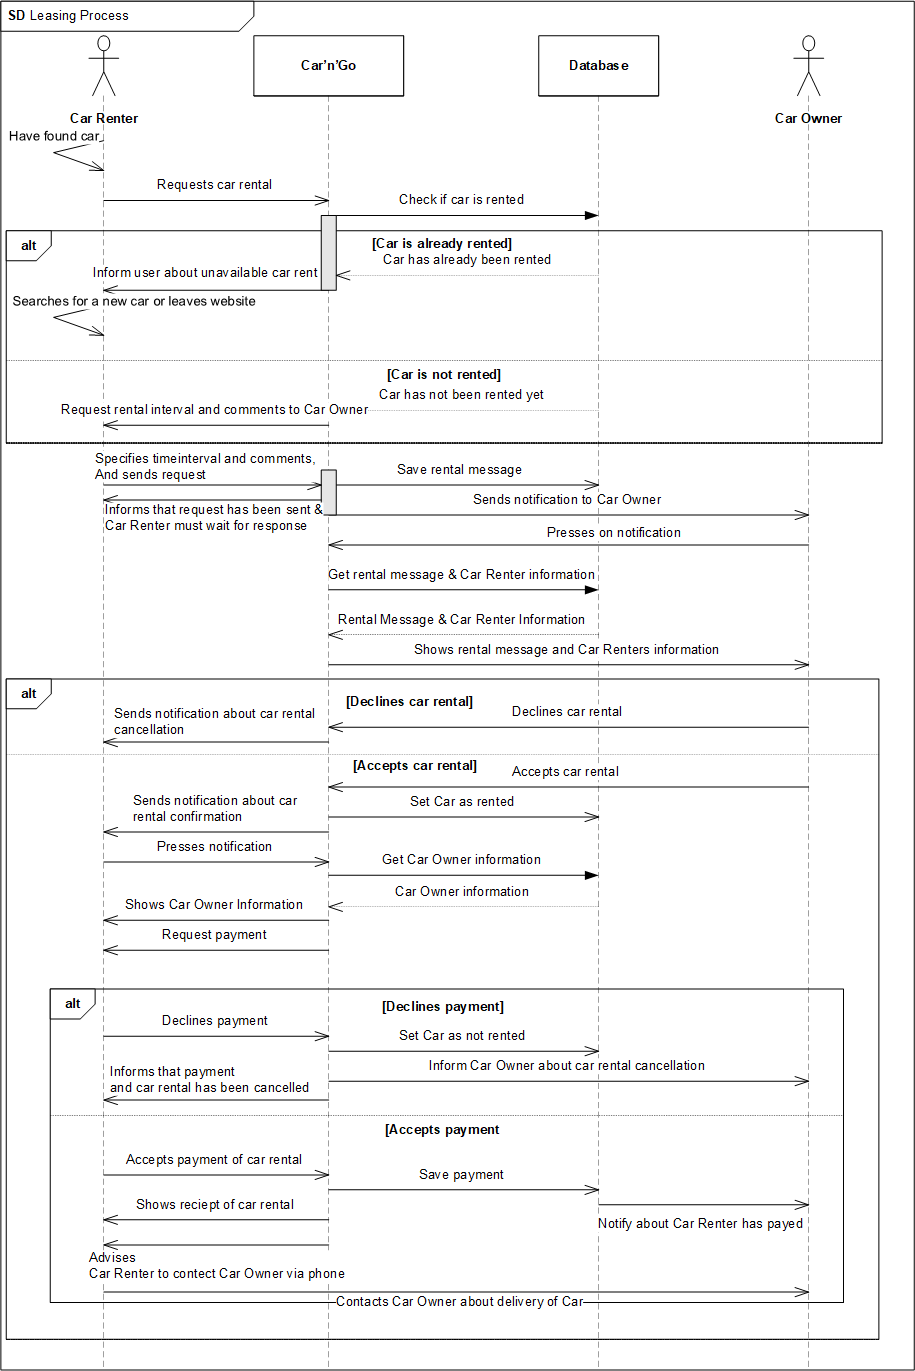
\includegraphics[width=1\textwidth]{Arkitektur/Softwarearkitektur/Leasing/graphics/Leasing_processSD.png}
    \caption{Sekvensdiagram for håndtering af udlejningsprocessen.}
    \label{fig:Leasing_processCD}
\end{figure}
Nedenfor ses applikationsmodellen, der også er lavet for udlejningsprocessen. Den inkluderer et klassediagram på figur \ref{fig:Leasing_processCD} og et statemachinediagram på figur \ref{fig:Leasing_processSTM}.
\begin{figure}[H]
    \centering
    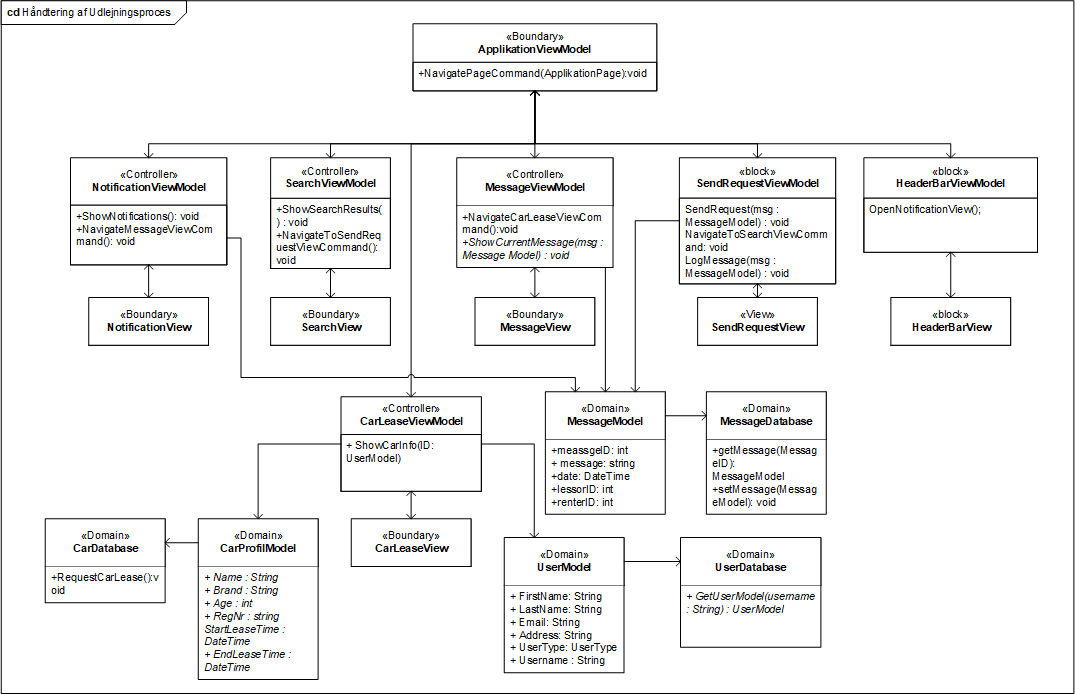
\includegraphics[width=1\textwidth]{Arkitektur/Softwarearkitektur/Leasing/graphics/Leasing_processCD.png}
    \caption{Klassediagram for håndtering af udlejningsprocessen.}
    \label{fig:Leasing_processCD}
\end{figure}

\begin{figure}[H]
    \centering
    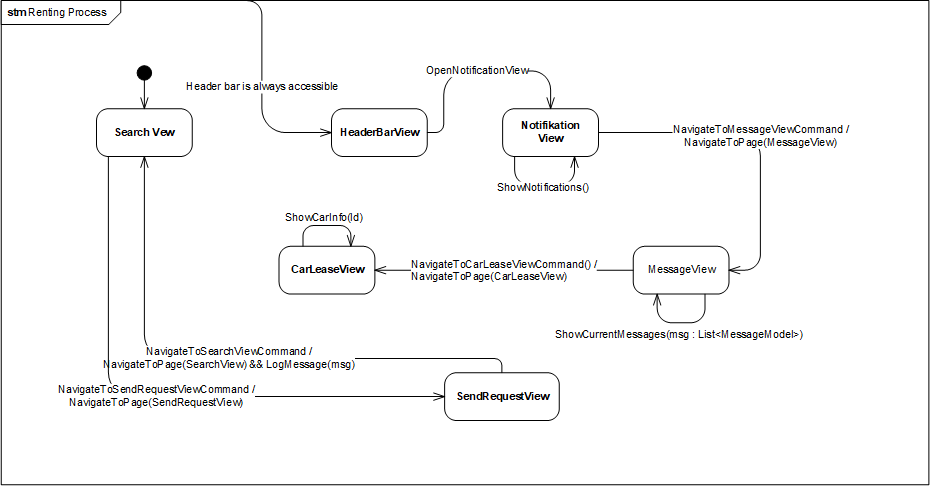
\includegraphics[width=1\textwidth]{Arkitektur/Softwarearkitektur/Leasing/graphics/Leasing_processSTM.png}
    \caption{Statmemachine for håndtering af udleningsprocessen. }
    \label{fig:Leasing_processSTM}
\end{figure}

\end{document}